%!TEX root = *.tex
%%%%%%%%%%%%%%%%%%
% メモ
\setlength{\baselineskip}{18pt}
\begin{comment}

\end{comment}
% カウンタのリセット
\setcounter{figure}{0}
% 解答
\qSentence{【解答】}
\begin{table}[htbp]
  \centering
  \begin{tabular}{lllll}
    ({\bf ア}) : $2mv_z$ & 
    ({\bf イ}) : $\dfrac{2L}{v_z}$ &
    ({\bf ウ}) : $\dfrac{v_z\varDelta t}{2L}$ &
    ({\bf エ}) : $\dfrac{m{v_z}^2\varDelta t}{L}$ & 
    ({\bf オ}) : $\dfrac{m}{L}$ \\
    ({\bf カ}) : $\dfrac{mN\overline{v^2}}{3L}$ &
    ({\bf キ}) : $\dfrac{mN\overline{v^2}}{3L^3}$ & 
    ({\bf ク}) : $\dfrac{3RT}{mN_A}$ &
    ({\bf ケ}) : $\dfrac{3}{2}\cdotp\dfrac{N}{N_A}RT$ \\
    \multicolumn{3}{l}{({\bf コ}) : $P(z)-P(z+\varDelta z)=d(z)g\varDelta z$} &
    \multicolumn{2}{l}{({\bf サ}) : $d(z)=\dfrac{mN_AP(z)}{RT}$} \\
    ({\bf シ}) : 6.4 & 
    ({\bf ス}) : $\dfrac{Nmg}{L^2}$ &
    ({\bf セ}) : $\dfrac{N_ANm^2g}{L^2RT}$
  \end{tabular}
\end{table}

\qSentence{【解説】}
\hang{(1)}
分子が壁面Aとの衝突時に受ける力積は$(-mv_z)-(mv_z)=-2mv_z$\unit{N$\cdotp$s} であるので,
壁面Aが受ける力積はその反作用力によるものであり,\underline{$2mv_z$}\unit{N$\cdotp$s} である.

\sethang{(1)}
分子は\z 軸方向に2L進む度に壁面Aと衝突するため,
\underline{$\tfrac{2L}{v_z}$}\unit{s} に1回衝突する.
すなわち,単位時間あたり$\tfrac{v_z}{2L}$回衝突する.
よって,$\varDelta t$\hspace{-0.3zw}\unit{s}の間に\underline{$\tfrac{v_z \varDelta t}{2L}$}\unit{回}衝突する.

\sethang{(1)}
衝突の度に壁面Aは$2mv_z$の力積を受けるので,$\varDelta t$の間に壁面Aが受ける力積は
\begin{align*}
  2mv_z \times \dfrac{v_z \varDelta t}{2L} = \underline{\dfrac{m{v_z}^2\varDelta t}{L}}\ \unit{N$\cdotp$s}
\end{align*}
である.時刻$\varDelta t$の間に壁面Aが力$f$を受けるとすると,その力積は$f\varDelta t$と表せるので,
\begin{align*}
  f\varDelta t &= \dfrac{m{v_z}^2\varDelta t}{L} \\
  \therefore \ f &= \underline{\dfrac{m{v_z}^2}{L}}\ \unit{N}
\end{align*}
となる.

\sethang{(1)}
$N$個の気体分子から壁面Aから受ける力$F$は各気体分子に対する$f$の総和である.
${v_z}^2$の平均値$\overline{{v_z}^2}$を用いて,
\begin{align*}
  F &= Nf =\frac{mN}{L} \times \overline{{v_z}^2} \ \unit{N}
\end{align*}
である.また,
\mbox{$\overline{v^2}=\overline{{v_x}^2}+\overline{{v_y}^2}+\overline{{v_z}^2}$},
\mbox{$\overline{{v_x}^2}=\overline{{v_y}^2}=\overline{{v_z}^2}$}より,$\overline{{v_z}^2}=\tfrac{\overline{v^2}}{3}$であるから,
\begin{align*}
  F &= \underline{\frac{mN\overline{v^2}}{3L}}
\end{align*}
さらに,壁面Aの面積は$L^2$\unit{$\text{m}^2$}なので,圧力を$P$とすると,
\begin{align*}
  F&= PL^2 \\
  \therefore P &= \underline{\frac{mN\overline{v^2}}{3L^3}}\ \unit{N/$\text{m}^2$}
\end{align*}
理想気体の状態方程式より
\begin{align*}
  PL^3 &= \dfrac{N}{N_A}RT \\
  \dfrac{1}{3}mN\overline{v^2} &= \dfrac{N}{N_A}RT \\
  \therefore \overline{v^2} &= \underline{\dfrac{3RT}{mN_A}}\ \unit{$\text{m}^2$/s$^2$}
\end{align*}

\sethang{(1)}
内部エネルギー$U$\unit{J}は$N$個の気体分子の運動エネルギーの総和であり,
\begin{align*}
  U&= N\times \dfrac{1}{2}m\overline{v^2} \\
  &= \underline{\dfrac{3}{2}\dfrac{N}{N_A}RT}\  \unit{J}
\end{align*}
である.

{%
\begin{wrapfigure}{r}{16zw}
  \vspace{-\intextsep}
  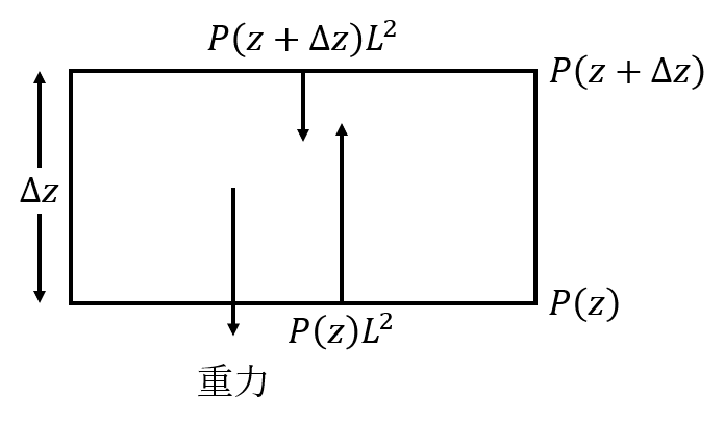
\includegraphics[width=16zw]{../graphs/jumon_65_sol.eps}
  \caption{}
  \label{fig:j65_sol}
\end{wrapfigure}
\hang{(2)}
高さ\z における厚さ$\varDelta z$の気柱にはたらく力のつりあいを考える.
この気柱の気体の密度は$d(z)$\unit{kg/$\text{m}^3$}と見なせるので,気体の質量は$d(z)\times L^2\varDelta z$\unit{kg}である.
よって力のつりあいは右図より,
\begin{align*}
  &P(z+\varDelta z)L^2 + d(z)L^2\varDelta zg = P(z)L^2 \\
  &\,\,\qquad\therefore \ \underline{P(z)-P(z+\varDelta z) = d(z)g\varDelta z}
\end{align*}

\sethang{(2)}
厚さ$\varDelta z$の気柱内の気体分子の数を$\varDelta N$とすると,理想気体の状態方程式より
\begin{align*}
  P(z)L^2\varDelta z = \dfrac{\varDelta}{N_A}RT\tag*{\ctext{1}}\label{eq:jotai}
\end{align*}
また,気体分子1個あたりの質量が$m$\unit{kg}なので,気柱内の気体分子の質量について
\begin{align*}
  m \varDelta N = d(z)L^2\varDelta z\tag*{\ctext{2}}\label{eq:mass}
\end{align*}
\ref{eq:jotai}と\ref{eq:mass}から,$\varDelta N$を消去して整理すると
\begin{align*}
  \underline{d(z) = \dfrac{mN_AP(z)}{RT}} \ \unit{kg/$\text{m}^3$}
\end{align*}

\sethang{(2)}
ここで,$P(z+\varDelta z)$が$P(z)$に比べ,0.010\%だけ小さいということは,
\begin{align*}
  \dfrac{P(z+\varDelta z)-P(z)}{P(z)} = -0.00010
\end{align*}
が成り立っている.求めた$P(z)-P(z+\varDelta z)$および$d(z)$を用いると,
\begin{align*}
  \dfrac{d(z)g\varDelta z}{P(z)} &= 1.0\times 10^{-4} \\
  \dfrac{mN_Ag\varDelta z}{RT} &= 1.0\times 10^{-4} \\
  \therefore\ \varDelta z &= \dfrac{RT}{mN_Ag}\times 1.0\times 10^{-4} \\
  \intertext{$mN_A$\unit{kg/mol}は気体1molあたりの質量であるから}
  \therefore\ \varDelta z &= \dfrac{8.3\times 300}{4.0\times 10^{-3}\times 9.8}\times 1.0\times 10^{-4}\\
  &= 6.35\cdots \\
  &= \underline{6.4\ \unit{m}}
\end{align*}

\sethang{(2)}
立方体容器全体(\ref{fig:j65_sol}で$\varDelta z=L$としたもの)の力のつりあいを考える.気体分子は$N$個あるので,はたらく重力は$N\times mg$であるから
\begin{align*}
  P(L)L^2 + Nmg &= P(0)L^2 \\
  \therefore\ P(0)-P(L) &= \underline{\dfrac{Nmg}{L^2}} \\
\end{align*}
$d(z)=\tfrac{mN_A}{RT}P(z)$より,両辺に$\tfrac{mN_A}{RT}$を掛けて
\begin{align*}
  \dfrac{mN_A}{RT}P(0)-\dfrac{mN_A}{RT}P(L) &= \dfrac{mN_A}{RT}\dfrac{Nmg}{L^2} \\
  \therefore\ d(0)-d(L) &= \underline{\dfrac{N_ANm^2g}{L^2RT}}
\end{align*}


\par}

%%%%%%%%%%%%%%%%%%
